\chapter{Il modello predittivo}\label{chap:modello}

Nel seguente capitolo affronteremo lo sviluppo del modello predittivo. 
Vedremo, prima di tutto, la struttura del modello discutendone i principali componenti e varie iterazioni di essa.  
In un secondo momento vedremo un problema fondamentale dato dalla distribuzione del dataset: il problema dello sbilanciamento.
Verrà anche introdotto brevemente come viene addestrato e le metriche utilizzato per valutarlo.
Infine saranno discussi i risultati ottenuti. 

\section{Struttura}
Come già introdotto nel \autoref{chap:introduzione_teorica}, questo modello si basa su un meccanismo di codifica del codice separato in due fasi:
    \begin{itemize}
        \item La prima codifica del \textit{code snippet} in un vettore di \textit{ast contexts}, effettuata a tempo di creazione del dataset, come già discusso nel \autoref{chap:dataset}.
        \item La seconda codifica del vettore di \textit{ast contexts} in un vettore di \textit{feature} attraverso meccanismi di \DL.
    \end{itemize}
Una volta ottenuto il vettore delle feature, vengono utilizzati due 'sotto reti' per la classificazione e la regressione. 
Possiamo vedere riassunta a grandi linee la struttura della rete in \autoref{fig:struttura}.

\begin{figure}[h]
    \centering
    \scalebox{0.8}{
        \begin{tikzpicture}[block/.style={draw, rectangle, minimum height=1cm}]
            \tikzset{vertex/.style = {shape=circle,draw,minimum size=1.5em}}
            \tikzset{edge/.style = {->,> = latex'}}
            
            \node[block, label={Input}] (input) at (0,0) {ast contexts vector};
            \node[block] (code2vec) at (4,0) {code2vec};

            \node[block] (classificazione) at (8, 2) {classificazione};
            \node[block] (regressione) at (8, -2) {regressione};
            
            \draw [edge] (input) to (code2vec);
            \draw [edge] (code2vec) to (classificazione);
            \draw [edge] (code2vec) to (regressione);
            
            \end{tikzpicture}
        }
      \caption{Struttura astratta del modello utilizzato}
      \label{fig:struttura}
\end{figure}

Nelle successive sezione discuteremo, in maniera approfondita, le seguenti tematiche:
    \begin{itemize}
        \item La struttura degli input e come sono stati gestiti i cambiamenti della loro forma discussi in precedenza nel \autoref{chap:dataset}.
        \item La struttura del modello di classificazione.
        \item La struttura del modello di regressione.
    \end{itemize}


\subsection{Struttura degli input}
Il dataset generato nel \autoref{chap:dataset} contiene per ogni suo elemento un vettore di \textit{ast contexts}, cioè un vettore di triple della forma:
    \[(x_s^{(i)}, p^{(i)}, x_t^{(i)})\]
tali per cui vale la seguente relazione:
    \[x_s^{(i)}, x_t^{(i)} \in \mathbb{N}^{l}, \quad p^{(i)} \in \mathbb{N}^{k}\]
dove $l$ e $k$ rappresentano rispettivamente la lunghezza massima del vettore dei token di inizio/fine e la lunghezza massima del vettore dei cammini\footnote{Nel caso in cui non siano effettivamente lunghi $l$ o $k$ vengono ridimensionati tramite del \textit{padding}},
fissate al momento della creazione del dataset (vedremo in seguito che valori sono stati assegnati e provati).


Prima però di poter utilizzare questo vettore come input del modello, deve essere trasformato in tre vettori separati della seguente forma:
\[x_s, x_t \in \mathbb{N}^{c \times l}, \quad p \in \mathbb{N}^{c \times k}\]
dove la constante $c$ rappresenta la lunghezza massima dei vettori di \textit{ast contexts} (di nuovo in seguito vedremo i suoi valori).
Definiamo i tre vettori nel seguente modo:
    \begin{align*}
        x_s &= (x_s^{(0)}, x_s^{(1)}, ..., x_s^{(c)}) \\
        x_t &= (x_t^{(0)}, x_t^{(1)}, ..., x_t^{(c)}) \\
        p &= (p^{(0)}, p^{(1)}, ..., p^{(c)}) 
    \end{align*}
Può succedere, però, che un vettore di \textit{ast contexts} abbia una lunghezza $c^{\prime} < c$.
In questo caso dovremo andare ad aggiungere $c - c^{\prime}$ \textit{ast contexts} di \textit{padding} che saranno rappresentati da specifiche triple di vettori di token che, nel rispettivo vocabolario, rappresentano dei token di \textit{padding} (saranno dei token \<PAD\textgreater).

Una volta fatto questo dobbiamo però indicare al modello quali degli \textit{ast contexts} sono di \textit{padding}. 
Per far ciò introduciamo l'ultimo dei quattro input del modello: la maschera.
La maschera sarà un vettore $m$ di lunghezza $c$ definito nel seguente modo:
    \begin{align*}
        m_i =
        \begin{cases*}
        1 & se l'elemento $i$-esimo non è padding \\
        0 & altrimenti
        \end{cases*}
    \end{align*}

\subsection{Gestione cambiamenti della forma}\label{subsec:cambiamenti_forma}
Una volta trasformato l'input avremo quindi tante quadruple della forma:
    \[(x_s, p, x_t, m)\]
tale per cui:
\[x_s, x_t \in \mathbb{N}^{c \times l}, \quad p \in \mathbb{N}^{c \times k}, \quad m \in  \mathbb{N}^{c}\]
All'interno del modello, la prima trasformazione che avviene è quella dell'\textit{embedding} dei tre vettori di token attraverso un \textit{layer} specifico.
Il risultato di ciò sono dei vettori della forma:
    \[x_s^{\prime}, x_t^{\prime} \in \mathbb{N}^{c \times l \times d}, \quad p^{\prime} \in \mathbb{N}^{c \times k \times d}\]
dove $d$ è la dimensione dell'\textit{embedding} (nota: $d$ può essere diverso per $p$, $x_s$ e $x_t$).
Nella studio di code2vec \cite{alon2019code2vec}, come era già stato discusso nel \autoref{chap:dataset}, i vettori d'input hanno una forma leggermente diversa:
\[x_s, x_t \in \mathbb{N}^{c}, \quad p \in \mathbb{N}^{c}, \quad m \in  \mathbb{N}^{c}\]
ottenendo successivamente al \textit{layer} di \textit{embedding}:
\[x_s^{\prime}, x_t^{\prime} \in \mathbb{N}^{c \times d}, \quad p^{\prime} \in \mathbb{N}^{c \times d}\]
Per uniformare quindi i valori a come quelli usati dalla ricerca, effettueremo un appiattimento dei vettori post-\textit{embedding}, ottenendo:
\[x_s^{\prime\prime}, x_t^{\prime\prime} \in \mathbb{N}^{c \times (l \cdot d)}, \quad p^{\prime\prime} \in \mathbb{N}^{c \times (k \cdot d)}\]


\subsection{Classificazione}
L'obbiettivo della classificazione in questo modello è il predire la classe di errore o l'assenza di errore. 
Il modello, di conseguenza, in output dovrà fornire un vettore $c$ tale per cui per ogni $i$:
\[0 \leq c_i \leq 1\]
avremo quindi che il vettore $c$ è una \textit{distribuzione di probabilità} delle classi da predire.
Di conseguenza la classe con maggior probabilità sarà la classe predetta, cioè:
    \[\argmax_i c_i\]
Nel lavoro svolto la rete di classificazione prenderà in input il vettore delle \textit{feature} prodotto dal modello di code2vec.
Questo vettore viene dato in input ad'una serie di \textit{hidden dense layer} culminanti in un \textit{layer} di predizione che utilizza come funzione di attivazione la funzione \textit{softmax}, andando a produrre il vettore $c$.

Visto l'output che produce questo modello, prima di poter computare la funzione di \textit{loss} dovremo trasformare il \textit{label} associato al \textit{code snippet} in una versione \textit{one-hot encoded}. 




\subsection{Regressione}
Il modello della regressione ha come scopo il predire il numero della riga dell'eventuale errore.
La struttura utilizzata è molto semplice: un unico \textit{dense layer} che prende in input il vettore delle \textit{feature} con un singolo output.

Similmente alla classificazione, anche per la regressione dobbiamo processare la riga dell'errore associata al \textit{code snippet}. 
Per evitare di avere una varianza troppo grande, con a volte numeri di riga molto bassi e a volte molto alti, il valore viene normalizzato da un fattore costante tale da rendere ogni singolo valore compreso tra 0 e 1.



\section{Sbilanciamento del dataset}\label{sec:sbilanciamento}
Illustriamo ora il problema principale in cui ci si è imbattuti nel realizzare questo modello: lo sbilanciamento del dataset.
Un dataset, in un problema di classificazione, si definisce sbilanciato se le proporzioni del numero di campioni per ogni classe hanno grosse differenze.
Nel nostro caso possiamo vedere ciò in \autoref{fig:sbilanciamento}. 
Come si può notare la classe dell'assenza di errori rappresenta circa il 95\% del dataset, mentre il restante 5\% è suddiviso fra le 16 classi possibili di errori.


\begin{figure}[h]
    \centering
    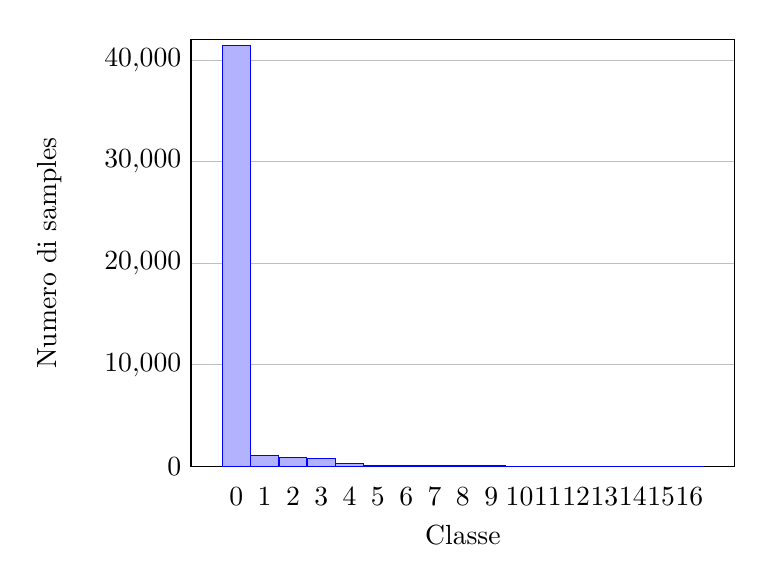
\begin{tikzpicture}
        \begin{axis}[
            width  = \textwidth * 0.7,
            height = 7cm,
            major x tick style = transparent,
            ybar=0.1pt,
            bar width=10pt,
            ymajorgrids = true,
            ylabel style={yshift=2ex},
            xlabel=Classe,
            ylabel=Numero di samples,
            xtick = data,
            scaled y ticks = false,
            ymin=0,ymax=42000,
            ytick style={draw=none},
            ]
    \addplot table {
      Classe Numero
      0 41417 
      1 1032
      2 911
      3 792
      4 325
      5 122
      6 85
      7 83
      8 80
      9 56
      10 31
      11 16    
      12 10
      13 4
      14 3
      15 2
      16 1      
    };
    \end{axis}
    \end{tikzpicture}

    \caption{Figura che mostra quanto il dataset sia sbilanciato sia verso la classe dell'assenza di errori sia internamente fra le classi di errori}
    \label{fig:sbilanciamento}
\end{figure}

Il problema dello sbilanciamento è molto grave poiché rende difficile sia l'addestramento della rete sia la sua valutazione, vediamo ora un esempio di ciò.
Supponiamo di creare un modello che predice, per ogni input datogli, sempre l'assenza di errore: col nostro dataset questo modello avrebbe una precisione del 95\%.
Vedendo solo questa metrica potrebbe quindi sembrare essere un modello quasi ideale, mentre invece ovviamente non lo è.
Vedremo nel \autoref{subsec:metriche} come esistono delle metriche in grado di essere utili nonostante lo sbilanciamento.

L'addestramento, invece, è reso difficile dal momento che, con le funzioni di \textit{loss} utilizzate, solitamente il modello tenderà a diventare come quello descritto sopra.
Verranno quindi utilizzate una serie di tecniche nel tentativo di ridurre gli effetti dello sbilanciamento, in particolare vedremo:
    \begin{itemize}
        \item L'utilizzo di una funzione di \textit{loss} pesata.
        \item L'utilizzo di \textit{oversampling}.
        \item La riduzione del numero di classi da predire. 
    \end{itemize}
Nell'addestramento del modello finale verranno utilizzate sia la seconda sia la terza tecnica.

\subsection{Loss pesata}
Il meccanismo di \textit{loss} pesata funziona in modo molto semplice: assegnare ad'ogni classe peso diverso nella computazione della \textit{loss}.
Facendo così, se si sono assegnati i pesi corretti, si avrà che le classi minoritarie avranno molto più peso rispetto a quelle maggioritarie e quindi, nel caso in cui il modello sbagli a predire una delle classi minoritarie, la perdita sarà maggiore.

In questo lavoro è stata implementata attraverso l'utilizzo di una \textit{matrice dei pesi} $W$ della forma:
    \[W \in \mathbb{R}^{n \times n}\]
dove $n$ rappresenta il numero di classi.
La semantica di questa matrice $W$ è la seguente: il valore $W_{i,j}$ indica il peso di un \textit{sample} di classe $i$ classificato erroneamente come di classe $j$. 
Definendo $f_i$ come la frequenza assoluta della classe $i$-esima, dovremo avere quindi che:
    \[W_{i,j} \propto \frac{f_j}{f_i}\]
Esistono diverse tecniche per assegnare questi pesi, in questo caso è stata utilizzata la seguente formula:
    \[W_{i,j} = \frac{f_j + \epsilon}{f_i + \epsilon}\]
L'aggiunta di un piccolo valore $\epsilon$ è dovuta al fatto che, in rari casi, $f_i = 0$.

\'E stato deciso di non utilizzare questo sistema poiché i risultati ottenuti non sono stati ottimali, infatti il modello, nei test effettuati, imparava in ogni caso a predire sempre la classe di assenza d'errore.
Una possibile spiegazione di ciò è che nonostante le classi minoritarie avessero un grosso peso, la probabilità di trovarle in un singolo \textit{batch} di addestramento era bassa, ciò implicava uno strano comportamento della funzione di \textit{loss}. 
 
\subsection{Oversampling}
L'\textit{oversampling} è il processo di aumentare artificialmente il numero di osservazioni delle classi minoritarie in modo tale da pareggiarle con quelle maggioritarie.
L'implementazione dell'\textit{oversampling} può avvenire in svariati modi:
    \begin{itemize}
        \item Ripetizione semplice delle osservazioni delle singole classi minoritarie.
        \item Creazione di osservazioni completamente nuove tramite metodi complessi. Un esempio di questo approccio è il metodo denominato \textit{smote}, descritto nella ricerca \cite{chawla2002smote}, che è fra i più popolari.
         Consiste nel creare dati nei segmenti che congiungono i $k$ vicini della medesima classe più vicini nel \textit{feature space}.
    \end{itemize}
In generale utilizzando questa tecnica avremo che l'addestramento del modello diventa più difficile poiché è più probabile che finisca in \textit{overfitting}.
Creando però dati completamente nuovi, ma teoricamente sensati, cioè come fa \textit{smote}, la probabilità di fare \textit{overfitting} è minore.

Nel caso di questo progetto non è stato possibile utilizzare \textit{smote} poiché l'implementazioni nelle librerie più comuni non funzionavano per la struttura dati usata.
Viene, invece, utilizzato il seguente metodo: ripetizione dei dati mischiando però l'ordine degli \textit{ast contexts} all'interno del vettore.
I due vantaggi ottenibile teoricamente tramite questa tecnica sono:
    \begin{itemize}
        \item Diminuire l'\textit{overfitting} riducendo il numero di dati uguali.
        \item L'eliminazione della semantica associata all'ordine degli \textit{ast contexts} all'interno di un vettore. Infatti, per come vengono estratti, l'ordine non ha alcuna importanza.
            Il riordinamento quindi potrebbe fare 'capire' ciò al modello.
    \end{itemize}

\subsection{Riduzione numero di classi}
L'ultima tecnica che andiamo ad'esporre è la riduzione del numero di classi da predire.
Questa tecnica trasforma il problema di classificazione a $n$ classi in un problema di classificazione a $k<n$ classi.
Una volta fissato un $k < n$ verranno determinate le $k - 1$ classi più frequenti (cioè con il numero di osservazioni più alto) e verranno scelte come le nuove classi.
Le restanti classi vengono aggregate in un'unica classe indicante un errore sconosciuto. 
Avremo, quindi, al variare di $k$ i seguenti casi:
    \begin{itemize}
        \item Ponendo $k=2$ avremo un problema di classificazione binaria, in cui viene classificato la presenza o assenza di errore.
        \item Ponendo $k=5$, come utilizzato in questo progetto, avremo la classificazione degli errori più comuni (\textit{memory leak}, \textit{null dereference}, \textit{dead store}), mentre il restante viene classificato come errore sconosciuto.
        \item Ponendo $k$ più vicino al valore di $n$ non avremo grossi cambiamenti.
    \end{itemize}
Possiamo vedere in \autoref{fig:riduzione} come al variare di $k$ cambia la distribuzione delle classi. 

Utilizzando questa tecnica insieme all'\textit{oversampling} si riduce significativamente l'\textit{overfitting}, poiché lo sbilanciamento del dataset è minore.

\begin{figure}[h]
    \centering
    \begin{subfigure}{.5\textwidth}
        \centering
        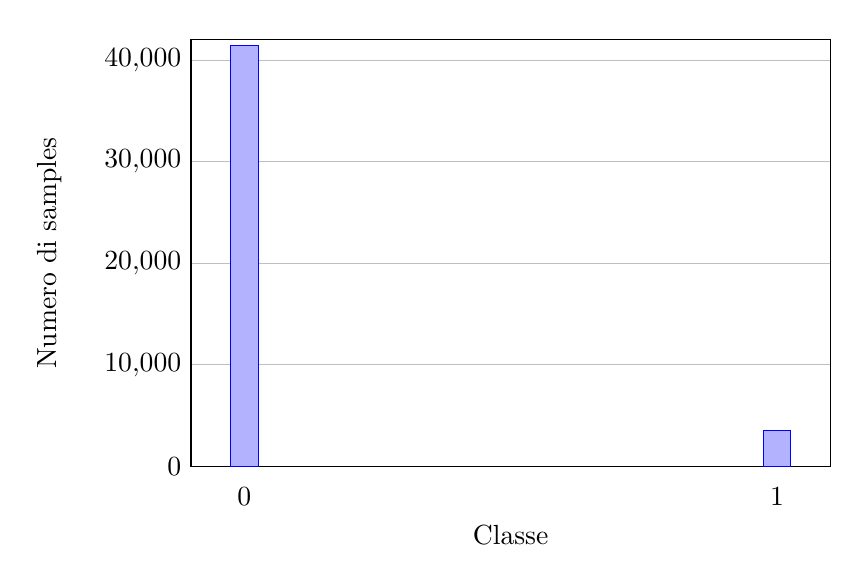
\begin{tikzpicture}
            \begin{axis}[
                width  = \textwidth * 0.8,
                height = 7cm,
                major x tick style = transparent,
                ybar=0.1pt,
                bar width=10pt,
                ymajorgrids = true,
                ylabel style={yshift=2ex},
                xlabel=Classe,
                ylabel=Numero di samples,
                xtick = data,
                scaled y ticks = false,
                ymin=0,ymax=42000,
                ytick style={draw=none},
                ]
                \addplot table {
                    Classe Numero
                    0 41417 
                    1 3553
                  };
        \end{axis}
        \end{tikzpicture}
    \caption{Riduzione del numero di classi a $k=2$}
    \end{subfigure}%
    \begin{subfigure}{.5\textwidth}
        \centering
        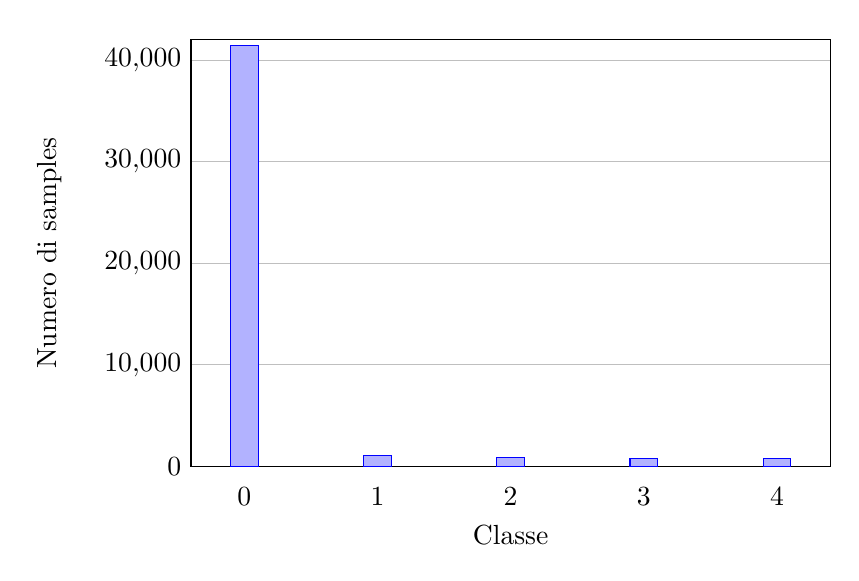
\begin{tikzpicture}
        \begin{axis}[
            width  = \textwidth * 0.8,
            height = 7cm,
            major x tick style = transparent,
            ybar=0.1pt,
            bar width=10pt,
            ymajorgrids = true,
            ylabel style={yshift=2ex},
            xlabel=Classe,
            ylabel=Numero di samples,
            xtick = data,
            scaled y ticks = false,
            ymin=0,ymax=42000,
            ytick style={draw=none},
            ]
            \addplot table {
                Classe Numero
                0 41417 
                1 1032
                2 911
                3 792
                4 818
              };
    \end{axis}
    \end{tikzpicture}

    \caption{Riduzione del numero di classi a $k=5$}
    \end{subfigure}


    \caption{Comparazione tra riduzione a $k=5$ e $k=2$ classi}
    \label{fig:riduzione}
\end{figure}
\pagebreak

\section{Addestramento}
L'addestramento della rete è stato eseguito numerose volte provando valori per gli \textit{iper parametri} ogni volta diversi. 
Questi parametri, nel nostro caso, consistono in:
    \begin{itemize}
        \item Gli iper parametri standard come \textit{learning rate, batch size, epochs, steps per epoch} e \textit{dropout rate} (per il \textit{layers} di \textit{dropout}).
        \item La dimensione degli \textit{embedding} dei token dei cammini e d'inizio/fine, cioè il valore $d$ introdotto in \autoref{subsec:cambiamenti_forma}.
        \item La dimensione del vettore delle \textit{feature} prodotto dal modello code2vec.
        \item Il numero $k$ di classi da utilizzare. 
    \end{itemize}
L'addestramento inoltre è stato eseguito utilizzando come ottimizzatore l'algoritmo Adam, descritto più in dettaglio in \cite{kingma2014adam}. 
Come \textit{loss function} ne vengono utilizzate due, una per la regressione e una per la classificazione, e sono le seguenti:
    \begin{itemize}
        \item La \textit{categorical crossentropy loss} per la classificazione, nel caso si utilizzi un $k>2$, mentre se $k=2$ si utilizza la \textit{binary crossentropy loss}.
        \item Per la regressione viene utilizzata la \textit{mean squared error}.
    \end{itemize}
Il dataset prima di essere utilizzato viene inoltre separato in tre insiemi distinti:
    \begin{itemize}
        \item Il \textit{train set} che è l'effettivo dataset con cui viene addestrata la rete. Questo rappresenta circa l'80\% del dataset intero.
        \item Il \textit{validation set} con cui, ad'ogni epoca, si va a valutare l'addestramento della rete. \Eaccentata{} fondamentale utilizzarlo poiché le metriche che si ottengo sul \textit{train set} non sono affidabili
                poiché la rete potrebbe (e farà) \textit{overfitting}. Questo rappresenta circa il 10\% del dataset.
        \item Il \textit{test set} con cui, a fine addestramento, si valuta di nuovo la rete. Come il \textit{validation set} rappresenta circa il 10\% del dataset.
    \end{itemize}
Requisito fondamentale è che questi tre insiemi devono essere distinti, e cioè non avere elementi in comune. 
Se avessero elementi in comune le metriche ottenute non sarebbero più affidabili. 

\subsection{Overfitting}\label{subsec:overfitting}
Un modello si dice che è in \textit{overfitting} quando si adatta troppo ai dati osservati e quindi perde capacità di generalizzazione.
In particolare nell'ambito del \ML{} e \DL{} succede quando il modello ha risultati molto buoni sul \textit{training set}, mentre significativamente peggiori sul \textit{validation} e \textit{test set}.

Possiamo vedere un esempio creando un modello che cerca di approssimare una funzione (cioè un problema di regressione). 
In \autoref{fig:esempi_overfitting_underfitting} possiamo vedere sia un modello in \textit{underfit} (cioè il contrario di \textit{overfit}), sia un modello ideale che ha approssimato correttamente la funzione e sia il modello in \textit{overfit}.
Se utilizzassimo quest'ultimo modello per predire nuovi valori, ad esempio determinando il valore di $f(x)$ dove $x$ non fa parte dei punti, non sarebbe in grado di generarne di corretti, mentre il modello ideale si.

\begin{figure}[h]
    \centering
    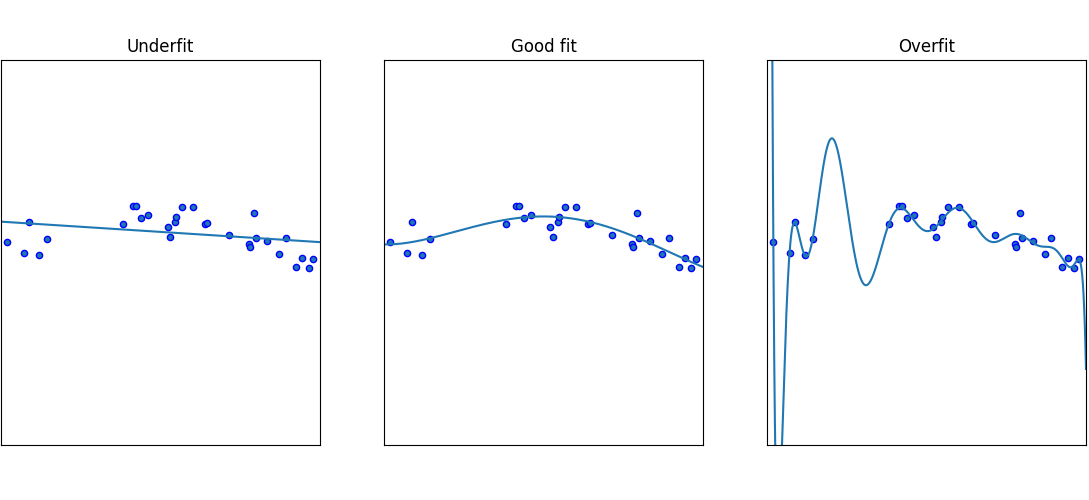
\includegraphics[scale=0.5]{images/esempio_overfitting_resize.png}
    \caption{Esempio di modello in stato di overfitting, underfitting e ottimale}
    \label{fig:esempi_overfitting_underfitting}
\end{figure}
Questo stato può essere causato da una serie di fattori:
    \begin{itemize}
        \item La complessità del modello, cioè il numero di parametri interni, è troppa alta rispetto al numero di osservazioni nel dataset.
        \item La fase di addestramento è stata eseguita per troppo tempo.
        \item Il dataset utilizzato per l'addestramento è troppo piccolo.
    \end{itemize}
Si può rilevare l'\textit{overfitting} guardando l'evoluzione della funzione di costo attraverso l'epoche di addestramento: nel caso in cui le \textit{loss} calcolate sul \textit{validation} e \textit{train set} divergono allora è molto probabile essere in \textit{overfitting}.
Vediamo un esempio di grafico che ci mostra la divergenza fra le due in \autoref{fig:overfitting_grafo_divergenza}

    \begin{figure}[h]
        \centering
        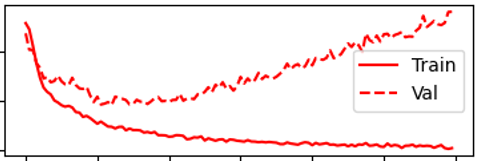
\includegraphics[scale=0.55]{images/LossOverfitting.png}
        \caption{Divergenza fra loss nel validation e train set}
        \label{fig:overfitting_grafo_divergenza}
    \end{figure}
Il modello utilizzato per questo lavoro soffre altamente di \textit{overfitting} e le cause sono principalmente la dimensione del dataset e la complessità del modello.
La prima causa è difficilmente eliminabile visto che andrebbe generato un nuovo dataset, mentre la seconda causa invece verrà affrontata riducendo valori come la dimensione degli \textit{embedding}, del vettore delle \textit{features} e degli input.
In particolare l'ultimo verrà fatto attraverso la riduzione dei valori di $c$, $l$ e $k$ introdotti in \autoref{subsec:cambiamenti_forma}.
Un'altra metodologia utilizzata per ridurlo è stato l'uso di specifici \textit{layers} di \textit{dropouts}.


\subsection{Metriche utilizzate}\label{subsec:metriche}
Le metriche sono un meccanismo fondamentale nella valutazione di un modello. 
Per questo progetto vengono utilizzate principalmente metriche per la classificazione, mentre per la regressione viene utilizzato solo il valore della funzione di costo.
In particolare vengono utilizzate le seguenti metriche:
    \begin{itemize}
        \item La precisione per ogni singola classe $i$ calcolata nel seguente modo:
            \[P_i = \frac{TP_i}{TP_i + FP_i}\]
            dove $TP_i$ e $FP_i$ rappresentano rispettivamente il numero di \textit{true positive} e \textit{false positive} per la classe $i$.             
            La precisione identifica quanti elementi classificati come di classe $i$ sono effettivamente di classe $i$.
        \item Il recall per ogni singola classe $i$, calcolato come:
            \[R_i = \frac{TP_i}{TP_i + FN_i}\]
            dove $FN_i$ rappresenta il numero di \textit{false negative} per la classe $i$.
            Il recall rappresenta quanti degli elementi della classe $i$ sono stati effettivamente individuati.
        \item L'f1-score per ogni classe $i$ che si calcola nel seguente modo:
            \[F1_i = \frac{2 \times P_i \times R_i}{P_i + R_i}\]
            e rappresenta la media armonica fra la precisione e il recall. Viene quindi utilizzata per bilanciare recall e precisione.
        \item L'f1-score globale calcolato come media degli f1-score delle singole classi.
        \item La matrice $M$ di confusione. Ogni elemento $M_{i,j}$ rappresenta il numero di volte in cui il modello ha predetto la classe $j$ mentre la classe vera era $i$.
         Le predizioni corrette sono quindi rappresentate nella diagonale, cioè quando $i=j$.
    \end{itemize}
Spesso succede che ci sia un \textit{trade off} tra la precisione e il recall.
In base al tipo di problema che si sta cercando di risolvere verrà prediletta una delle due metriche.
In questo lavoro è stato deciso di prediligere il recall, poiché è, a nostro avviso, più importante essere in grado di rilevare tutti i possibili errori.

\section{Risultati}
\subsection{Risultati dati dal test dataset}
\subsection{Risultati dati su codice creato al momento}



\section{Ulteriore architettura per la classificazione provate}
Come vedremo in seguito, il modello riesce a determinare con sufficiente correttezza se un \textit{code snippet} presenta o no un errore e riesce a catalogare bene il tipo di errore.
Se però deve fare queste predizioni tutte insieme (e cioè deve predire o la classe indicante l'assenza di errore o la classe dell'errore), vedremo, il modello non generalizzerà altrettanto bene.

Per provare a migliorare i risultati del modello, è stato provato a dividere il meccanismo di predizioni in due fasi:
    \begin{itemize}
        \item Determinare la presenza o l'assenza di un errore.
        \item Determinare la classe dell'errore.
    \end{itemize}
In questa modalità qui, quindi, il modello oltre ad'effettuare le regressione esegue due classificazioni: una binaria e una a più classi.

I risultati prodotti da questa versione, però, non sono così distanti dal modello effettivamente usato.
Questo potrebbe essere determinato da un fattore principale: la difficoltà nell'addestramento. 
Infatti, indipendentemente dalla predizione binaria che fa, il modello restituirà sempre in output anche una predizione sulla classe dell'errore e di conseguenza verrà computata la funzione di perdita.
Per questa ragione anche ai frammenti di codice senza errori bisogna associare un vettore per la predizione delle classi, ma dati i problemi dovuti allo sbilanciamento del dataset discussi in \autoref{sec:sbilanciamento},
il modello imparava a predire solo questo vettore (che è sicuramente il più prevalente).

Una possibile miglioria sarebbe di separare completamente i due modelli: uno predice la presenza o no di errori e l'altro predice solamente l'errore e il numero della riga.
Il funzionamento sarebbe poi il seguente: si utilizza il primo modello per primo poi, nel caso di rilevamento di errori, si utilizza il secondo modello per determinarne il tipo.
Non è stata esplorata questa possibilità poiché al di fuori della portata di questo lavoro. 

\section{Utilizzo}